\apendice{Documentación técnica de programación}

\section{Introducción}

En este apartado se describe la documentación técnica de programación del proyecto. El objetivo es explicar la organización interna de la aplicación y facilitar su mantenimiento o ampliación futura por parte de otros desarrolladores.

El proyecto consiste en una aplicación web educativa orientada al aprendizaje del algoritmo C4.5. La aplicación incluye diferentes módulos relacionados con el cálculo de entropía, entropía condicional, elección de nodos, construcción paso a paso del árbol de decisión y poda posterior del árbol generado.

A nivel técnico, la aplicación está desarrollada principalmente con HTML, CSS y JavaScript. No dispone de un servidor propio, por lo que la lógica de carga, validación, cálculo y visualización se ejecuta directamente en el navegador del usuario. Los datasets utilizados por el simulador se almacenan en archivos CSV y pueden ser seleccionados desde la propia aplicación o cargados localmente por el usuario.

El módulo principal del proyecto es el simulador del árbol C4.5, que permite construir árboles de decisión a partir de datasets mixtos con atributos numéricos, categóricos y booleanos. Además, ofrece una visualización SVG del árbol, tablas de cálculo, navegación paso a paso, controles de zoom y una vista específica para estudiar el procedimiento de poda.

\section{Estructura de directorios}

A continuación se describe la estructura principal de directorios y archivos del proyecto, indicando la finalidad de cada parte.

\begin{itemize}
    \item \textbf{applications:} contiene las diferentes páginas y módulos funcionales de la aplicación web.
    \begin{itemize}
        \item \textbf{index.html:} página principal de la aplicación. Actúa como menú de acceso a los distintos módulos disponibles.

        \item \textbf{code.js:} archivo JavaScript auxiliar utilizado por la página principal.

        \item \textbf{css:} contiene los estilos generales utilizados en la página principal de la aplicación.
        \begin{itemize}
            \item \textbf{style.css:} hoja de estilos común de la portada.
        \end{itemize}

        \item \textbf{img:} contiene imágenes utilizadas dentro de la aplicación web, como el fondo y el logotipo de la Universidad de Burgos.

        \item \textbf{lib:} contiene librerías y funciones compartidas por distintos módulos.
        \begin{itemize}
            \item \textbf{jquery-3.7.1.min.js:} librería jQuery utilizada por las páginas de la aplicación.
            \item \textbf{entropy-calculator.js:} funciones auxiliares relacionadas con el cálculo de entropía.
            \item \textbf{funcionesCalcAlgC45.js:} funciones de cálculo utilizadas en el contexto del algoritmo C4.5.
            \item \textbf{input-check.js:} funciones de validación de entradas.
        \end{itemize}

        \item \textbf{entropia:} módulo dedicado al cálculo y explicación de la entropía.
        \begin{itemize}
            \item \textbf{index.html:} página del módulo de entropía.
            \item \textbf{css/styles.css:} estilos propios del módulo.
            \item \textbf{js/calculator.js:} lógica principal de cálculo.
            \item \textbf{js/classNumHandler.js:} gestión del número de clases introducidas por el usuario.
            \item \textbf{lib/d3.v7.min.js:} librería D3.js utilizada para visualizaciones.
            \item \textbf{test:} pruebas asociadas a este módulo.
        \end{itemize}

        \item \textbf{entropia condicional:} módulo dedicado al cálculo de entropía condicional.
        \begin{itemize}
            \item \textbf{index.html:} página del módulo.
            \item \textbf{css/styles.css:} estilos propios.
            \item \textbf{js/calculator.js:} lógica del cálculo de entropía condicional.
            \item \textbf{js/catNumHandler.js:} gestión dinámica de categorías y valores.
            \item \textbf{test:} pruebas asociadas al módulo.
        \end{itemize}

        \item \textbf{Elección de nodo:} módulo dedicado a la simulación del proceso de selección de un nodo del árbol.
        \begin{itemize}
            \item \textbf{index.html:} página del módulo de elección de nodo.
            \item \textbf{styles.css:} estilos específicos del módulo.
            \item \textbf{js/classNumHandler.js:} gestión de clases.
            \item \textbf{js/csvHandler.js:} carga y tratamiento de datos en formato CSV.
            \item \textbf{js/dataTable.js:} generación y actualización de tablas de datos.
            \item \textbf{js/stepbystep.js:} lógica de la simulación paso a paso.
        \end{itemize}

        \item \textbf{Arbol C4.5:} módulo principal de construcción y poda del árbol de decisión C4.5.
        \begin{itemize}
            \item \textbf{index.html:} página de simulación de construcción del árbol C4.5.
            \item \textbf{poda.html:} página dedicada a la simulación del procedimiento de poda.
            \item \textbf{styles.css:} estilos específicos del módulo del árbol.
            \item \textbf{datasets:} datasets CSV de ejemplo y metadatos asociados.
            \item \textbf{js/c45.mjs:} implementación principal del algoritmo C4.5, validación de filas, cálculo de entropía, ganancia de información, \textit{Split Info}, \textit{Gain Ratio}, construcción del árbol, generación de pasos y poda.
            \item \textbf{js/datasetHandler.js:} gestión de la interfaz del simulador, carga de CSV, renderizado de tablas, árbol SVG, controles de navegación, zoom y vista de poda.
            \item \textbf{js/workspacePanels.js:} gestión de los paneles desplegables del espacio de trabajo.
        \end{itemize}
    \end{itemize}

    \item \textbf{tests:} contiene pruebas automáticas de la lógica principal del algoritmo C4.5.
    \begin{itemize}
        \item \textbf{c45.test.mjs:} pruebas sobre entropía, \textit{Split Info}, \textit{Gain Ratio}, validación de datasets, atributos numéricos, atributos categóricos y construcción de árboles.
    \end{itemize}

    \item \textbf{doc:} contiene documentación del proyecto.
    \begin{itemize}
        \item \textbf{Estructura de la web:} documento con información sobre la estructura de la aplicación.
    \end{itemize}

    \item \textbf{img:} contiene imágenes generales del proyecto, como el logotipo institucional.

    \item \textbf{.github:} contiene la configuración de GitHub.
    \begin{itemize}
        \item \textbf{workflows/github-actions-deploy.yml:} flujo de GitHub Actions encargado del despliegue automático en GitHub Pages.
    \end{itemize}
\end{itemize}

\section{Manual del programador}

En esta sección se describe la implementación de las partes principales de la aplicación web, incluyendo la carga y validación de datos, la construcción del árbol de decisión mediante el algoritmo C4.5, la generación de la simulación paso a paso, el procedimiento de poda y la representación visual del árbol.

\subsection{Estructura general del proyecto}

El proyecto está organizado como una aplicación web de cliente, desarrollada principalmente con HTML, CSS y JavaScript. No existe un servidor propio para procesar los datos, por lo que la carga de archivos, la validación, los cálculos del algoritmo y la visualización se realizan directamente en el navegador.

La carpeta principal de la aplicación es \texttt{applications}. Dentro de ella se encuentran los distintos módulos docentes:

\begin{itemize}
    \item \texttt{entropia}: módulo dedicado al cálculo y explicación de la entropía.
    \item \texttt{entropia condicional}: módulo dedicado al cálculo de la entropía condicional.
    \item \texttt{Elección de nodo}: módulo que simula la selección de atributos mediante las métricas utilizadas en C4.5.
    \item \texttt{Arbol C4.5}: módulo principal de construcción del árbol de decisión y simulación de poda.
    \item \texttt{lib}: funciones y librerías compartidas por varios módulos.
    \item \texttt{img}: recursos gráficos utilizados por la aplicación.
\end{itemize}

El módulo principal se encuentra en \texttt{applications/Arbol C4.5}. Este directorio contiene dos páginas HTML principales: \texttt{index.html}, encargada de la simulación de construcción del árbol, y \texttt{poda.html}, encargada de la visualización del procedimiento de poda. Ambas páginas utilizan la misma lógica JavaScript principal.

Los archivos más relevantes del módulo son los siguientes:

\begin{description}
    \item[\texttt{c45.mjs}:] contiene la implementación principal del algoritmo C4.5, incluyendo la validación de filas, el cálculo de entropía, la evaluación de atributos, la construcción recursiva del árbol, la generación de pasos y el procedimiento de poda.
    \item[\texttt{datasetHandler.js}:] gestiona la interacción con la interfaz, la carga de datasets, la lectura de archivos CSV, el renderizado de tablas, el dibujo del árbol SVG, los controles de navegación y la visualización de la poda.
    \item[\texttt{workspacePanels.js}:] gestiona el comportamiento de los paneles retráctiles del área de trabajo.
    \item[\texttt{datasets}:] contiene los datasets CSV de ejemplo y el archivo \texttt{dataInfo.js}, donde se almacena información descriptiva y enlaces asociados a dichos datasets.
    \item[\texttt{styles.css}:] define los estilos específicos del módulo del árbol C4.5.
\end{description}

Además, el directorio \texttt{tests} contiene el archivo \texttt{c45.test.mjs}, que agrupa pruebas automáticas sobre la lógica principal del algoritmo C4.5.

\subsection{Estructuras de datos principales}

La implementación no define clases específicas para representar el árbol, sino que utiliza objetos JavaScript creados dinámicamente. La función principal \texttt{buildC45FromRows()} devuelve un objeto que contiene el árbol construido, los pasos de simulación, las cabeceras del dataset, las clases detectadas, la información de poda y el criterio de selección utilizado.

El nodo base se crea mediante la función \texttt{createBaseNode()}. Los campos más relevantes de cada nodo son:

\begin{description}
    \item[\texttt{id}:] identificador numérico del nodo.
    \item[\texttt{attribute}:] nombre del atributo seleccionado en el nodo. En las hojas toma el valor \texttt{null}.
    \item[\texttt{attributeType}:] tipo del atributo, con valores como \texttt{numeric} o \texttt{categorical}.
    \item[\texttt{threshold}:] umbral seleccionado cuando el atributo es numérico.
    \item[\texttt{gain}:] ganancia de información de la división seleccionada.
    \item[\texttt{splitInfo}:] valor de \textit{Split Info}.
    \item[\texttt{gainRatio}:] valor de \textit{Gain Ratio}.
    \item[\texttt{conditionalEntropy}:] entropía condicional de la división.
    \item[\texttt{entropy}:] entropía del subconjunto de datos asociado al nodo.
    \item[\texttt{n}:] número de registros que llegan al nodo.
    \item[\texttt{classCounts}:] objeto que almacena el número de registros de cada clase.
    \item[\texttt{isLeaf}:] valor booleano que indica si el nodo es una hoja.
    \item[\texttt{predictedLabel}:] clase mayoritaria asociada al nodo o a la hoja.
    \item[\texttt{parent}:] referencia al nodo padre.
    \item[\texttt{children}:] array con los nodos hijo.
    \item[\texttt{branchCondition}:] condición que conecta el nodo con su padre.
    \item[\texttt{dataRowIndexes}:] índices de las filas del dataset que llegan al nodo.
    \item[\texttt{depth}:] profundidad del nodo dentro del árbol.
    \item[\texttt{x}, \texttt{y}:] coordenadas utilizadas para representar visualmente el nodo en el SVG.
\end{description}

Las ramas no se almacenan como objetos independientes, sino como información dentro del campo \texttt{branchCondition} de cada hijo. Este campo contiene, entre otros, el atributo utilizado, el operador de comparación, el valor o umbral y la etiqueta que se muestra en la rama.

Los pasos de simulación se generan mediante \texttt{collectSteps()}. Cada paso contiene:

\begin{description}
    \item[\texttt{stepNumber}:] número de paso.
    \item[\texttt{treeElementId}:] identificador visual del nodo u hoja.
    \item[\texttt{type}:] tipo de elemento, con valores \texttt{node} o \texttt{leaf}.
    \item[\texttt{node}:] referencia al nodo asociado al paso.
    \item[\texttt{dataRowIndexes}:] filas del dataset implicadas en el paso.
    \item[\texttt{activeConditions}:] condiciones acumuladas desde la raíz hasta el nodo actual.
    \item[\texttt{valueTableData}:] datos de evaluación utilizados para construir la tabla de cálculos.
\end{description}

La poda se almacena en el campo \texttt{pruning} del modelo. Este objeto incluye el árbol podado, los pasos de visualización, las evaluaciones realizadas y los datos necesarios para mostrar el proceso de poda de forma incremental.

\subsection{Implementación del algoritmo C4.5}

La construcción del árbol comienza a partir de los datos cargados desde el CSV. En primer lugar, se identifica la cabecera del conjunto de datos, se toma la última columna como clase objetivo y se determinan los atributos disponibles para la construcción del modelo.

El algoritmo construye el árbol de forma recursiva. En cada nodo se analiza el subconjunto de registros correspondiente, se calcula la distribución de clases, la entropía y la clase mayoritaria. A continuación, se evalúan los atributos disponibles para seleccionar la mejor división.

Los atributos categóricos se dividen según sus distintos valores, generando una rama para cada categoría. En cambio, los atributos numéricos se ordenan y se analizan mediante posibles umbrales de división. Estos umbrales se generan entre valores consecutivos cuando se produce un cambio de clase, separando los registros en dos grupos.

Para cada posible división se calculan las métricas necesarias: entropía condicional, ganancia de información, \textit{Split Info} y \textit{Gain Ratio}. El criterio principal utilizado por el algoritmo C4.5 es el \textit{Gain Ratio}, aunque la aplicación también permite emplear la ganancia de información como alternativa didáctica. En ese caso, la interfaz muestra un aviso indicando que el criterio original del algoritmo C4.5 es la razón de ganancia.

Una vez seleccionada la mejor división, se crean las ramas correspondientes y el proceso se repite sobre cada subconjunto generado. Si el atributo seleccionado es categórico, este deja de estar disponible en las ramas inferiores. Si el atributo es numérico, puede volver a utilizarse posteriormente con otros umbrales. El procedimiento continúa hasta que se cumple alguna condición de parada y se genera una hoja con la clase correspondiente.


\subsection{Implementación de estructura de SVG}

Antes de explicar el cálculo de la posición de cada nodo, debe mencionarse que el árbol se crea utilizando elementos SVG de HTML. En la página web se coloca un contenedor SVG, cuyo tamaño cambia dinámicamente cuando se redimensiona la ventana del navegador.

En la figura \ref{Fig_D.1} se muestra el objeto SVG creado tanto para las lineas como para los nodos/ramas en la web.

\begin{figure}[htbp]
     \centering
     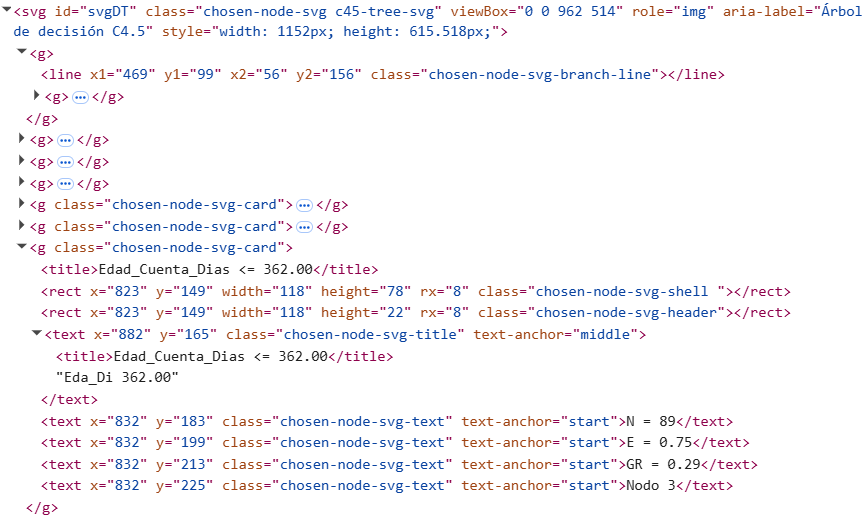
\includegraphics[width=0.75\textwidth]{img/Representacion_SVG_Nodo_Linea.png}
     \caption{Ejemplo visual del elemento del SVG en la web}
     \label{Fig_D.1}
 \end{figure}

\subsubsection{Cálculo de la posición de los nodos}

La posición de los nodos del árbol se calcula antes de generar la representación SVG. Esta lógica se encuentra en la función \texttt{assignTreePositions()}, que asigna a cada nodo unas coordenadas \texttt{x} e \texttt{y}. Estas coordenadas se almacenan en el propio objeto del nodo y posteriormente son utilizadas por la función de renderizado para dibujar nodos y ramas.

En primer lugar, se definen tres parámetros principales:

\begin{description}
    \item[\texttt{spacingX}:] separación horizontal entre hojas consecutivas.
    \item[\texttt{spacingY}:] separación vertical entre niveles del árbol.
    \item[\texttt{minCanvasWidth}:] anchura mínima utilizada para centrar árboles pequeños.
\end{description}

La coordenada vertical de cada nodo se calcula directamente a partir de su profundidad. El nodo raíz se sitúa en la parte superior del SVG y cada nivel inferior se desplaza verticalmente una cantidad fija. De esta forma, todos los nodos que pertenecen al mismo nivel del árbol comparten una posición vertical similar.

La coordenada horizontal se calcula de forma recursiva. El procedimiento comienza recorriendo el árbol desde la raíz, pero la posición definitiva de un nodo interno depende de la posición de sus hijos:

\begin{itemize}
    \item Si el nodo es una hoja, se coloca en la siguiente posición horizontal disponible. Para ello se utiliza un contador incremental de hojas, de modo que cada nueva hoja queda separada de la anterior por \texttt{spacingX}.
    \item Si el nodo tiene hijos, primero se calculan recursivamente las posiciones de todos ellos.
    \item Una vez posicionados los hijos, el nodo padre se coloca en el punto medio entre el hijo situado más a la izquierda y el hijo situado más a la derecha.
\end{itemize}

De esta manera, las hojas quedan distribuidas de izquierda a derecha y cada nodo interno aparece centrado sobre el conjunto de ramas que dependen de él. Esta estrategia reduce visualmente el solapamiento y facilita seguir la estructura jerárquica del árbol. En la figura \ref{Fig_D.2} se muestra una imagen de como quedaría el árbol después de haber puesto las hojas finales.

\begin{figure}[htbp]
     \centering
     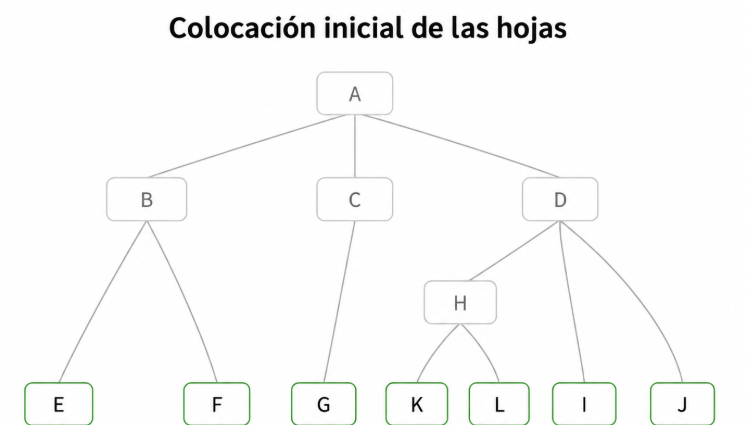
\includegraphics[width=0.75\textwidth]{img/Colocacion_Inicial_Hojas.png}
     \caption{Ejemplo visual de como quedaría el árbol en primera instancia}
     \label{Fig_D.2}
 \end{figure}


Tras asignar las posiciones iniciales, se ejecuta la función \texttt{centerCompactTree()}. Esta función recopila todos los nodos del árbol, calcula la coordenada horizontal mínima y máxima, y obtiene la anchura real ocupada por la estructura. Si el árbol es más estrecho que la anchura mínima definida, se desplazan todos los nodos horizontalmente para que la raíz quede centrada dentro del área de visualización. En la figura \ref{Fig_D.3} se muestra una imagen de como quedaría el árbol después de que se ejecutara la función previa.

\begin{figure}[htbp]
     \centering
     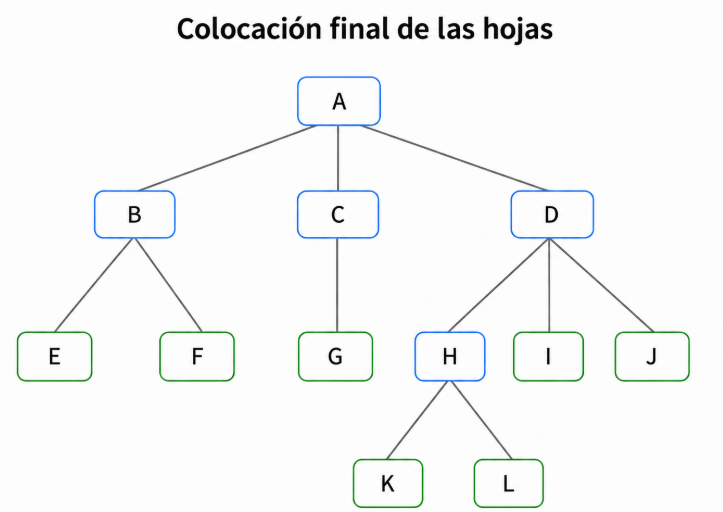
\includegraphics[width=0.75\textwidth]{img/Colocacion_Final_Hojas.png}
     \caption{Ejemplo visual de como quedaría el árbol finalmente}
     \label{Fig_D.3}
 \end{figure}


\subsection{Implementación del procedimiento de poda}

La poda se realiza una vez construido el árbol completo. Su objetivo es simplificar la estructura del árbol eliminando aquellos subárboles que no aportan una mejora suficiente en la clasificación.

El procedimiento recorre el árbol desde las hojas hacia la raíz. Para cada nodo interno se evalúa el subárbol que depende de él y se compara con una versión simplificada en la que todo ese subárbol se sustituye por una única hoja con la clase mayoritaria del nodo.

El error estimado de cada hoja se calcula mediante la siguiente expresión:


Error_{hoja} = \frac{E + 0.5}{N}


donde (E) representa el número de registros mal clasificados por la hoja y (N) el número total de registros que llegan a ella.

A partir de los errores de las hojas se calcula el error estimado total del subárbol mediante una media ponderada. Después, se calcula el error que tendría la hoja simplificada si el subárbol completo se sustituyera por una única hoja.

Si el error estimado de la hoja simplificada es menor o igual que el error estimado del subárbol, se aplica la poda y el subárbol se reemplaza por una hoja. En caso contrario, se conserva la estructura original.

Además, durante este proceso se almacena la información necesaria para mostrar la poda paso a paso, como el nodo evaluado, las hojas implicadas, los errores calculados y la decisión tomada en cada caso.


\section{Compilación, instalación y ejecución del proyecto}

No existen ejecutables ni \textit{scripts} que deban ejecutarse para iniciar este proyecto, ya que está basado en páginas HTML con archivos JavaScript, que actúan como \textit{scripts} encargados de hacer interactivas las páginas web. Sin embargo, para poder utilizar las librerías incluidas localmente en el proyecto, es necesario clonarlo desde el repositorio de GitHub.

El proyecto fue desarrollado en un equipo con sistema operativo Windows 11. Para trabajar con él, es necesario tener Git instalado en el equipo, lo cual puede hacerse descargando el instalador desde la página web oficial de Git \footnote{Git download for Windows: \url{https://www.git-scm.com/download/win}}

El proyecto debe clonarse en el sistema de archivos del usuario. A partir de ese momento, no es necesario realizar ningún proceso adicional de compilación ni instalación.

Sin embargo, para ejecutar los \textit{tests} incluidos en el proyecto, es necesario tener instalados Node.js y npm, lo cual puede realizarse de varias formas, tal y como se indica en la página web oficial de Node.js \footnote{Instalación de Node.js y npm: \url{https://docs.npmjs.com/downloading-and-installing-node-js-and-npm}}. Para instalar las dependencias necesarias del entorno de pruebas, se debe ejecutar el comando \texttt{npm install} desde la terminal. El directorio actual debe ser la carpeta del proyecto en el sistema de archivos del usuario. Una vez instaladas todas las dependencias, los \textit{tests} pueden ejecutarse mediante el comando \texttt{npm test}.


\section{Pruebas del sistema}

Para comprobar la funcionalidad principal del algoritmo C4.5 se ha utilizado el módulo de pruebas nativo de Node.js, denominado \texttt{node:test}.

Las pruebas específicas del algoritmo C4.5 se encuentran en el archivo \texttt{tests/c45.test.mjs}. En este fichero se comprueban funciones relevantes de la implementación, como el cálculo de la entropía, el cálculo de \textit{Split Info}, el cálculo de \textit{Gain Ratio}, la detección de valores numéricos, la validación de datasets, la generación de umbrales para atributos numéricos y la construcción de árboles con atributos categóricos, numéricos y booleanos.

Estas pruebas pueden ejecutarse desde la raíz del proyecto mediante el siguiente comando:

\begin{verbatim}
node --test tests/c45.test.mjs
\end{verbatim}

El uso de \texttt{node:test} resulta adecuado para este módulo porque el algoritmo C4.5 está implementado como un módulo JavaScript independiente en \texttt{c45.mjs}, lo que permite probar su lógica sin depender de la interfaz gráfica ni del navegador. No obstante, las pruebas no cubren todos los comportamientos visuales de la aplicación, como el renderizado SVG, los controles de zoom o la interacción con los paneles, que requieren validación manual en el navegador.